\chapter{Wprowadzenie}

Aby dobrze przedstawić problemy i algorytmy będące tematem pracy, niezbędne jest przytoczenie podstawowych pojęć oraz zagadnień odnoszących się NP-zupełności.

Podstawowym pojęciem, które w pierwszej kolejności należało by przedstawić jest samo pojęcie "problemu". Według definicji w [1] problem abstrakcyjny $Q$ jest relacją dwuargumentową, określoną na zbiorze $I$ egzemplarzy problemu oraz zbiorze $S$ rozwiązań problemu. Egzemplarzem jest struktura matematyczna, natomiast podzbiór jej elementów składowych jest rozwiązaniem. Przenosząc to na przykład dla problemu MAXIMUM-INDEPENDET-EDGE-SET (czyli znalezienia maksymalnego skojarzenia) egzemplarzem jest graf $G$ złożony ze zbioru wierzchołków $V$ oraz krawędzi $E$. Zatem maksymalny zbiór krawędzi nie mających wspólnych wierzchołków jest rozwiązaniem tego problemu. Skoro problem jest relacją, a nie funkcją możliwa jest sytuacja, że dla jednego egzemplarza może istnieć wiele rozwiązań.

W przypadku poruszania się w obrębie teorii NP-zupełności takie definiowanie problemu jest zbyt ogólne dlatego najlepiej jest ograniczyć się do problemów decyzyjnych. W tej formie znana jest instancja problemu oraz wynik będący odpowiedzią. W przypadku INDEPENDET-EDGE-SET egzemplarz ma postać $i = <G,k>$ , a rozumiemy go: w grafie $G$ istnieje skojarzenie o mocy co najmniej $k$. Rozwiązaniem jest podzbiór zbioru krawędzi $E' \in E$ o mocy co najmniej $k$. Zadnie polega na zweryfikowaniu czy podany wynik jest rzeczywiście prawdziwy. Nie trudno zauważyć że dla tak postawionego problemu zbiór odpowiedzi w takim przypadku ogranicza się do dwóch wartości prawdy lub fałszu. Pozornie łatwe podejście w celu rozpatrywania problemu nie jest wcale takie proste gdy dochodzi do jego realizacji.
	
Inną formą podejścia do problemu jest podejście optymalizacyjne. Podobnie jak w problemie decyzyjnym na wstępie otrzymujemy instancje problemu, jednak nie występuje sugerowane rozwiązanie. Naszym zadaniem jest teraz znalezienie najlepszego wyniku, w zależności czy nasz zbiór wynikowy chcemy minimalizować ( w celu zmniejszania pewnych kosztów) czy też zależy nam na maksymalizowaniu ( w celu zwiększenia pewnych zysków). Odpowiedzą tak sformułowanemu problemowi będzie moc zbioru wynikowego, czasami również elementy tego zbioru. Mimo iż optymalizacyjne podejście wydaję się przy realizacji trudniejsze, można je łatwo zastąpić formą decyzyjną w bardzo prosty sposób. Należy obrać początkową trywialną wartość, a następnie zmieniać ją o jednostkową wartość do momentu aż przestanie istnieć rozwiązanie dla naszej wartości. W przypadku minimalizacji za trywialną wartość obieramy maksymalną wartość dla zbioru, którą później dekrementujemy. Natomiast dla maksymalizacji trywialną wartością startową jest zero, które zwiększamy aż do momentu w którym przestanie istnieć rozwiązanie.

Większa część problemów należy do klasy złożoności P, dlatego rzadko podejmuje się problemy wybiegające poza tę klasę. Problemy będące tematem tej pracy wybiegają dalej i dotyczą sławnej hipotezy: "czy P $\ne$ NP", dlatego obszar który podejmuje praca odnosi się do klas problemów P, NP i NPC. Praca zakłada że P $\ne$ NP w innym przypadku wywód ten nie ma sensu.%to ostatnie zdanie jest tu potrzebne ?

Najbardziej powszechna klasa P zawiera ten zbiór problemów dla których istnieje algorytm znajdujący rozwiązanie w czasie wielomianowym. Oznaczymy czas działania algorytmu jako funkcje $f$ która będzie działać ze zbioru oznaczającego rozmiar danych o ustalonym kodowaniu na zbiór odpowiadający liczbie operacji elementarnych potrzebnych do zakończenia działania algorytmu. Przy tak określonej funkcji jeśli możemy ją ograniczyć z góry przez dowolną funkcję wielomianową $O(nk)$ to wtedy problem należy do klasy złożoności P.

O ile P $\ne$ NP to klasa NP zawiera te problemy które są "weryfikowalne" w czasie wielomianowym. Przez słowo "weryfikowalne" rozumiemy, że istnieje takie świadectwo pozytywne (zwane inaczej dowodem), dzięki któremu jesteśmy w stanie sprawdzić czy otrzymane rozwiązanie jest poprawne. Jak widać klasa P $\subseteq$ NP z tej racji iż jeśli możemy rozwiązać problem w czasie wielomianowym to również jesteśmy w stanie w wielomianowym czasie sprawdzić pozytywność świadectwa.

Klasa NPC jest tym co różni klasę P i NP, w jej skład wchodzą te problemy które należą do NP a nie należących do P. Nasuwa się pytanie: "Czy w ogóle istnieją takie problemy z klasy NP, których nie można rozwiązać w czasie wielomianowym?". Na obecny stan rzeczy odpowiedz brzmi: nie wiadomo. W czasie powstawania pracy nikt dotąd nie udowodnił że wszystkie problemy $Q\in$ NP są rozwiązywalne w czasie wielomianowym, ani też nie pokazał że istniej taki problem z klasy NPC który nie jest rozwiązany w czasie wielomianowym. Tematem tej pracy właśnie są te problemy o których wiem że są weryfikowalne w czasie wielomianowym, a nie są rozwiązywalne w czasie wielomianowym.

\begin{figure}[tbh]
\centering
\begin{multicols}{2}
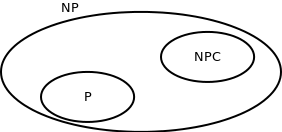
\includegraphics[width=0.75\hsize]{definitions/P_neq_NP.png}
\caption{P $\neq$ NP $\land$ NPC $\neq\emptyset$}
\label{P_neq_NP}
\columnbreak
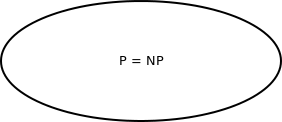
\includegraphics[width=0.75\hsize]{definitions/P_eq_NP.png}
\caption{P $=$ NP $\land$ NPC $=\emptyset$}
\label{P_eq_NP}
\end{multicols}
\end{figure}


Szczególną własnością problemów NPC jest że jeśli choć jeden problem znajdzie się w klasie P to wszystkie problemy z klasy NPC będą należały do klasy P. Pokazuje to że jeśli komuś uda się znaleźć algorytm wielomianowy rozwiązujący jakikolwiek problem z klasy NPC to oznaczało by że P $=$ NP. Związanie ze sobą tych wszystkich problemów NPC zawdzięczamy redukcji wielomianowej, polega ona na tym że rozwiązanie pewnego problemu można sprowadzić do rozwiązania innego. Odbywa się to za pośrednictwem algorytmu redukcji, który jest w stanie przeprowadzić każdą instancję problemu $A$ do postaci instancji problemu $B$ w czasie wielomianowym. Aby to zobrazować posłużę się trywialnym przykładem w którym problem $Q$ obliczenia długości wektora w $\mathbb{R}^{2}$ zredukujemy do problemu $Q'$ obliczenia długości wektora w $\mathbb{R}^{3}$. Mając tak zdefiniowane problemy potrzebujemy jeszcze algorytm redukcji. Nasz algorytm będzie rozszerzał wektor o trzecią pozycję i wpisywał w to miejsce $0$. Teraz każdy wektor z $\mathbb{R}^{2}$ możemy przedstawić w $\mathbb{R}^{3}$ a następnie obliczyć jego długość. Widać że długości wektora $[x1,x2,0]$ odpowiada długości wektora $[x1,x2]$. Pokazuje to że problem $Q$ można zredukować do problemu $Q'$.

Mimo iż tak wiele wiadomo o problemach NP-zupełnych to nadal sprawiają one wyzwanie. O ile algorytmy o złożoności większej od wielomianowej potrafią znaleźć optymalne rozwiązanie, o tyle należy mieć pewność, że dane będą z odpowiednio wąskiego zakresu. Jeśli jednak zakres danych jest zbyt duży pozostaje jedynie heurystyczne poszukiwanie wyniku dla mocno sprecyzowanego problemu lub zadowolenie się wynikiem zbliżonym do optymalnego w oparciu o algorytm aproksymacyjny. W przypadku heurystycznego podejścia nie można za wiele powiedzieć gdyż wszystko zależy od indywidualnej potrzeby o którą musi zadbać algorytm  oraz improwizacji na którą można sobie pozwolić.

Obecnie najbardziej popularną metodą jest wykorzystanie algorytmów aproksymacyjnych ze względu na ich wielomianową złożoność. Jakość takiego algorytmu zależy od znalezionego rozwiązania $C$ względem rozwiązania optymalnego $C^{*}$. Współczynnik aproksymacji $1 \leq \rho(n)$ jest wyznacznikiem jakości i ogranicza z góry stosunek kosztów: $max(\dfrac{C}{C^{*}},\dfrac{C^{*}}{C}) \leq \rho(n)$

Wzór ten uwzględnia przypadek maksymalizacji jak i minimalizacji określając ile razy otrzymane rozwiązanie jest gorsze od optymalnego. Dla maksymalizacji mamy $0 \leq C \leq C^{*}$ czyli wartość znalezionego rozwiązania jest nie większa od rozwiązania optymalnego. Natomiast w problemie minimalizacji $0 \leq C^{*} \leq C$ wartość znalezionego rozwiązania jest nie mniejsza od rozwiązania optymalnego.
